\textsl{}\documentclass[pdftex]{beamer}
\usetheme{Frankfurt}

% declare the path(s) where your graphic files are
% ../.. is the GeocronDocuments directory
\graphicspath{{../../images/external/location_routing/}{../../images/diagrams/}}
\DeclareGraphicsExtensions{.pdf,.png}

%some screwiness required to get the apalike bib style working
\usepackage{natbib}
\def\newblock{\hskip .11em plus .33em minus .07em}

\begin{document}


% Show the ToC at the start of each section, with the current section highlighted
\AtBeginSection[]
{
   \begin{frame}
        \frametitle{Roadmap}
        \tableofcontents[currentsection]
   \end{frame}
}

\title[FT Comm. MW]{Fault-Tolerant Middleware: Communication}
\subtitle{Reliable communication middelwares for distributed systems}
\author[K. Benson]{Kyle E. Benson}
\institute[UCI]{
  Department of Computer Science\\
  University of California, Irvine\\
  Irvine, California 92697\\[1ex]
  \texttt{kebenson@uci.edu}
}


\begin{frame}[plain]
	\titlepage
\end{frame}

% Breaking intro into its own part suppresses navigation bar info
\part{intro}

\begin{frame}{Introduction}

\begin{itemize}
	\item Traditional routing
	\begin{itemize}
		\item Unique address: IP, MAC, Peer ID, etc.
		\item Source routing: next hop address, neighbor index
		\item Local routing: distance-vector, link state, label-switching
	\end{itemize}
	
	\pause
	\item Why location information?
	\begin{itemize}
		\item Geocast: message all (or some) nodes in target region
		\item Latency: request from closer server, route locally when possible
		\item Congestion: confine route requests to smaller regions (MANETs)
		\item Energy: closer nodes need less radio power to reach
		\item Sensors: regional event detection, spatial querying
		\item Planning: paths (robots), surveillance cameras (focus on area target will appear next)
		\alert<3>{\item Recovery: avoid problematic areas of the network}
		\begin{itemize}
		\alert<3>{\uncover<3>{\item our primary interest!}}
		\end{itemize}
	\end{itemize}
\end{itemize}

\end{frame}

% % % % % % % % % % % % % % % % % % % % % % % % % % % % % % % % % % % % % % % % % %
\part{rest}

\begin{frame}{Roadmap}
	\tableofcontents
\end{frame}

\section{Location Service}

\begin{frame}{Location Service}
\begin{columns}
\begin{column}{.5\textwidth}

	\begin{itemize}
		\item Nodes have GPS
		\item But how to look up destination's location?
		\item Maintain global information \uncover<2->{\alert{easily outdated/inefficient}}
		\item<3-> Distribute load
		\begin{itemize}
			\item In \cite{Li:2000:SLS:345910.345931}, node updates \emph{location servers} (LS) throughout network
			\item Divide network into hierarchical grid
			\item LS's in 3 external grids at each level
			\item Lookup distance $<$ square LS co-resides in
		\end{itemize}
		
	\end{itemize}

\end{column}

\begin{column}{.5\textwidth}
\uncover<3->{
\begin{figure}
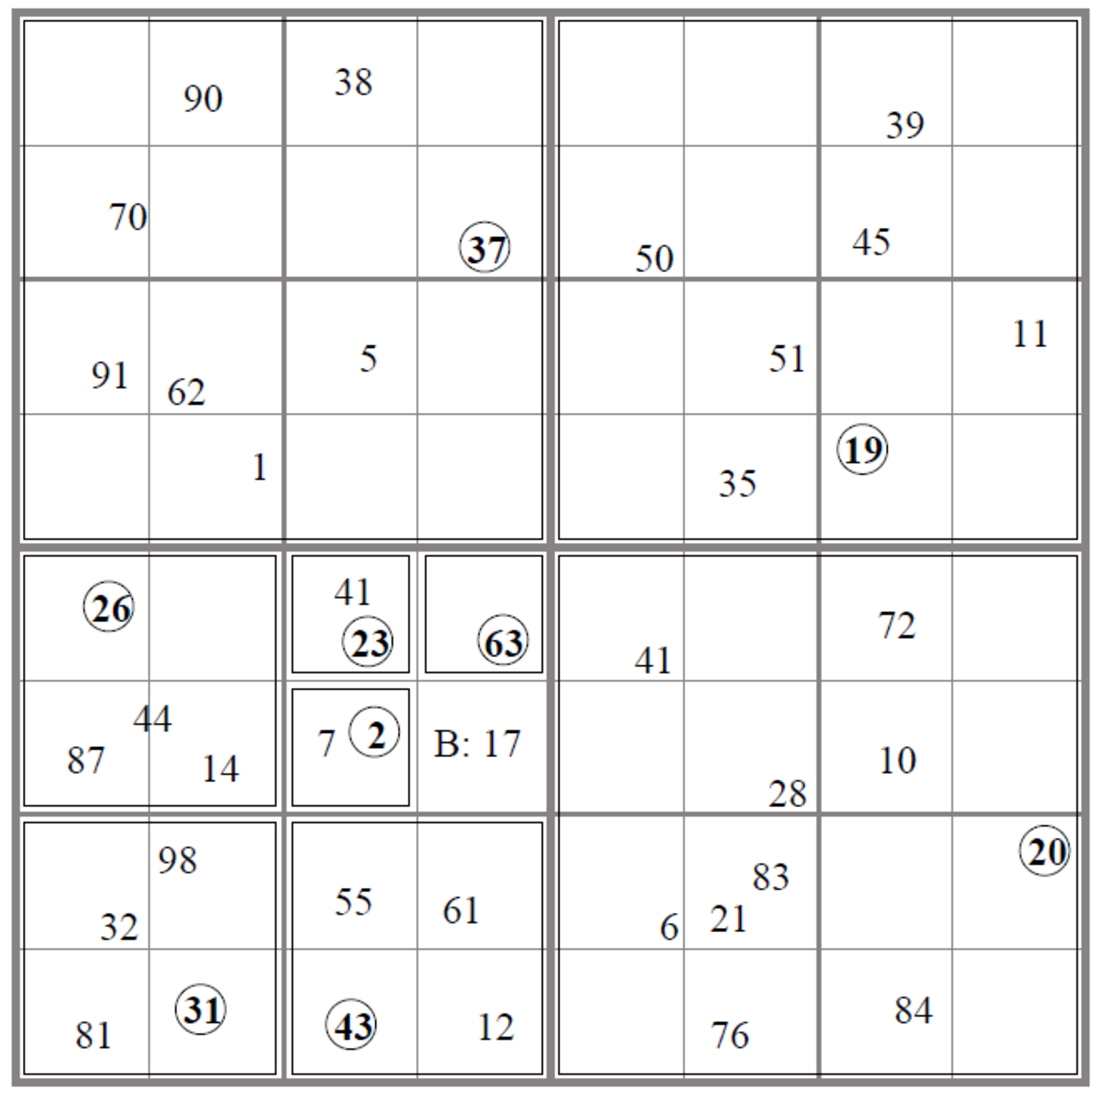
\includegraphics[width=\textwidth]{location_service}
\caption{Hierarchical grid with 4 order-i squares in order-i+1 square.}
\end{figure}}
\end{column}
\end{columns}
\end{frame}


\end{document}
